\documentclass[tikz]{standalone}
\usetikzlibrary{shapes,arrows.meta}
\begin{document}
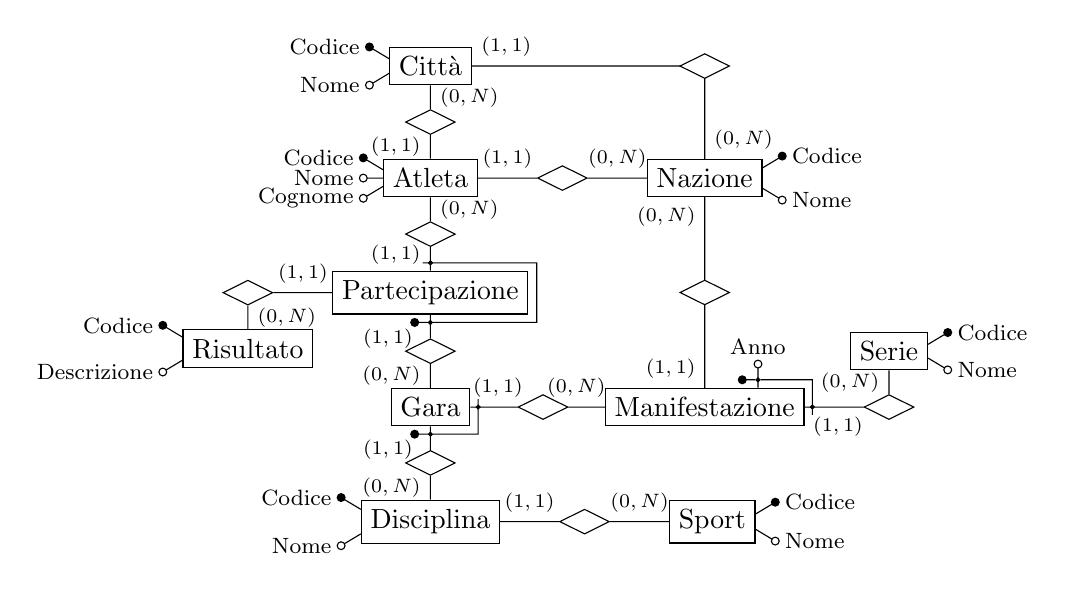
\begin{tikzpicture}
    \draw

    %%* Attributi:
    %%  node[draw, circle, inner sep=1pt, fill=black]{}node[right]{\footnotesize A}
    %%? Distanza orizzontale: E -(0.25,0.x)- A
    %%? Distanza verticale: E -(0,x * 0.22)- A

    %%* Cardinalità:
    %%  node[below right]{\scriptsize $(0,N)$}
    %%  node[above right]{\scriptsize $(0,N)$}
    %%  node[midway, above]{\scriptsize $(0,N)$}

    %%* Relazione:
    %%  node[draw, diamond, shape aspect=2, inner sep=3pt, anchor=90](r1){}
    %%  node[draw, diamond, shape aspect=2, inner sep=0.2pt, anchor=180](r2){R2}

    %%* Entità:
    %%  node[draw, rectangle, anchor=90](e1){}
    %%? Distanza verticale: E -(0.3)- R -(0.3) E
    %%? Distanza orizzontale: E -(0.75)- R -(0.75)- E

    %%* Città
    (0,0)node[draw, rectangle, anchor=180](e1){Città}
    (e1.270)--++(0,-0.3)node[draw, diamond, shape aspect=2, inner sep=3pt, anchor=90](r1){}node[midway, right]{\scriptsize $(0,N)$}

    
    (e1.190)--++(-0.25,-0.15)node[draw, circle, inner sep=1pt, fill=white]{}node[left]{\footnotesize Nome}
    (e1.170)--++(-0.25,0.15) node[draw, circle, inner sep=1pt, fill=black]{}node[left]{\footnotesize Codice}


    %%* Atleta
    (r1.270)--++(0,-0.3)node[draw, rectangle, anchor=90](e2){Atleta}node[midway, left]{\scriptsize $(1,1)$}
    (e2.0)--++(0.75,0)node[draw, diamond, shape aspect=2, inner sep=3pt, anchor=180](r2){}node[midway, above]{\scriptsize $(1,1)$}
    (e2.270)--++(0,-0.3)node[draw, diamond, shape aspect=2, inner sep=3pt, anchor=90](r3){}node[midway, right]{\scriptsize $(0,N)$}

    
    (e2.190)--++(-0.25,-0.15)node[draw, circle, inner sep=1pt, fill=white]{}node[left]{\footnotesize Cognome}
    (e2.180)--++(-0.25,0)node[draw, circle, inner sep=1pt, fill=white]{}node[left]{\footnotesize Nome}
    (e2.170)--++(-0.25,0.15) node[draw, circle, inner sep=1pt, fill=black]{}node[left]{\footnotesize Codice}



    %%* Nazione
    (r2.0)--++(0.75,0)node[draw, rectangle, anchor=180](e3){Nazione}node[midway, above]{\scriptsize $(0,N)$}
    (e3.90)node[above right]{\scriptsize $(0,N)$}|-(e1.0)node[above right]{\scriptsize $(1,1)$}node[midway, draw, diamond, shape aspect=2, inner sep=3pt, fill=white](r4){}

    (e3.350)--++(0.25,-0.15)node[draw, circle, inner sep=1pt, fill=white]{}node[right]{\footnotesize Nome}
    (e3.10)--++(0.25,0.15) node[draw, circle, inner sep=1pt, fill=black]{}node[right]{\footnotesize Codice}

    %%* Partecipazione
    (r3.270)--++(0,-0.2)node[midway, left]{\scriptsize $(1,1)$}node[draw, circle, inner sep=0.5pt, fill=black](a){}--++(0,-0.1)node[draw, rectangle, anchor=90](e6){Partecipazione}
    (e6.180)--++(-0.75,0)node[draw, diamond, shape aspect=2, inner sep=3pt, anchor=0](r6){}node[midway, above]{\scriptsize $(1,1)$}
    (e6.270)--++(0,-0.1)node[draw, circle, inner sep=0.5pt, fill=black](b){}--++(0,-0.2)node[draw, diamond, shape aspect=2, inner sep=3pt, anchor=90](r7){}

    (a)++(-0.1,0)--++(1.45,0)|-(b)--++(-0.2,0)node[draw, circle, inner sep=1pt, fill=black]{}

    %%* Risultato
    (r6.270)--++(0,-0.3)node[draw, rectangle, anchor=90](e7){Risultato}node[midway, right]{\scriptsize $(0,N)$}

    (e7.190)--++(-0.25,-0.15)node[draw, circle, inner sep=1pt, fill=white]{}node[left]{\footnotesize Descrizione}
    (e7.170)--++(-0.25,0.15) node[draw, circle, inner sep=1pt, fill=black]{}node[left]{\footnotesize Codice}


    %%* Gara
    (r7.90)++(-0.1,0)node[left]{\scriptsize $(1,1)$}
    (r7.270)--++(0,-0.3)node[draw, rectangle, anchor=90](e8){Gara}node[midway, left]{\scriptsize $(0,N)$}
    (e8.0)--++(0.1,0)node[draw, circle, inner sep=0.5pt, fill=black](a){}--++(0.5,0)node[draw, diamond, shape aspect=2, inner sep=3pt, anchor=180](r8){}node[midway, above]{\scriptsize $(1,1)$}
    (e8.270)--++(0,-0.1)node[draw, circle, inner sep=0.5pt, fill=black](b){}--++(0,-0.2)node[draw, diamond, shape aspect=2, inner sep=3pt, anchor=90](r9){}

    (a)++(0,0.1)|-(b)--++(-0.2,0)node[draw, circle, inner sep=1pt, fill=black]{}

    %%* Manifestazione
    (r8.0)-|(e3.270)node[midway,draw, rectangle, fill=white](e9){Manifestazione}
    (r8.0)++(0.1,0)node[above]{\scriptsize $(0,N)$}

    ;\draw[line width=0mm](e3.270)node[below left]{\scriptsize $(0,N)$}--(e9.90)node[above left]{\scriptsize $(1,1)$}node[midway,draw, diamond, shape aspect=2, inner sep=3pt, thin, fill=white](r10){};\draw

    (e9.0)--++(0.1,0)node[draw, circle, inner sep=0.5pt, fill=black](a){}--++(0.65,0)node[draw, diamond, shape aspect=2, inner sep=3pt, anchor=180](r11){}node[midway, below]{\scriptsize $(1,1)$}

    (e9.20)--++(0,0.1)node[draw, circle, inner sep=0.5pt, fill=black](b){}--++(0,0.2)node[draw, circle, inner sep=1pt, fill=white]{}node[above]{\footnotesize Anno}

    (a)++(0,-0.1)|-(b)--++(-0.2,0)node[draw, circle, inner sep=1pt, fill=black]{}


    %%* Serie
    (r11.90)--++(0,0.3)node[draw, rectangle, anchor=270](e10){Serie}node[midway, left]{\scriptsize $(0,N)$}

    (e10.350)--++(0.25,-0.15)node[draw, circle, inner sep=1pt, fill=white]{}node[right]{\footnotesize Nome}
    (e10.10)--++(0.25,0.15) node[draw, circle, inner sep=1pt, fill=black]{}node[right]{\footnotesize Codice}


    %%* Disciplina
    (r9.90)++(-0.1,0)node[left]{\scriptsize $(1,1)$}
    (r9.270)--++(0,-0.3)node[draw, rectangle, anchor=90](e4){Disciplina}node[midway, left]{\scriptsize $(0,N)$}
    (e4.0)--++(0.75,0)node[draw, diamond, shape aspect=2, inner sep=3pt, anchor=180](r5){}node[midway, above]{\scriptsize $(1,1)$}

    (e4.190)--++(-0.25,-0.15)node[draw, circle, inner sep=1pt, fill=white]{}node[left]{\footnotesize Nome}
    (e4.170)--++(-0.25,0.15) node[draw, circle, inner sep=1pt, fill=black]{}node[left]{\footnotesize Codice}

    %%* Sport
    (r5.0)--++(0.75,0)node[draw, rectangle, anchor=180](e5){Sport}node[midway, above]{\scriptsize $(0,N)$}

    
    (e5.350)--++(0.25,-0.15)node[draw, circle, inner sep=1pt, fill=white]{}node[right]{\footnotesize Nome}
    (e5.10)--++(0.25,0.15) node[draw, circle, inner sep=1pt, fill=black]{}node[right]{\footnotesize Codice}


    ;
\end{tikzpicture}
\end{document}